\documentclass[11pt, professionalfonts]{beamer}
\usetheme[
	% sectionpage=progressbar,
	% subsectionpage=progressbar,
	progressbar=head]{metropolis}

\useoutertheme{infolines}
% \useinnertheme{rounded}
\usecolortheme{beaver}



\usepackage{longtable}
\usepackage{newtxtext,newtxmath}
\usepackage[backend=biber,style=gb7714-2015, gbnamefmt=lowercase, 
maxcitenames=2,
mincitenames=1, 
gbcitelocal=gb7714-2015,
gbpub=false,
doi=false,
isbn=false,
url=false,
eprint=false]{biblatex}
\addbibresource{yy.bib}
\hypersetup{pdfpagemode=FullScreen}
\usepackage{ctex}
\setmainfont{Times New Roman}
\setCJKmainfont[ItalicFont=华文楷体,BoldFont=华文细黑]{华文宋体}
\usepackage{graphicx}
\usepackage{amsmath}
\usepackage{amsfonts}
\usepackage{subfigure}
\usepackage{url}
\definecolor{awesome}{rgb}{1.0, 0.13, 0.32}
% \usepackage{mathptm}
\numberwithin{equation}{section}
\usefonttheme[onlymath]{serif}
% \setlength{\parskip}{1.2em}
\DeclareGraphicsExtensions{.eps,.ps,.jpg,.bmp,.png}

\author{统计71~~王泽昊}
\institute{指导教师: 张春霞}

\date{2021年4月21日}

\title{数学与统计学院~毕业设计}
\subtitle[本科毕业设计]{聚类算法在地震速度谱自动拾取中的应用研究}

\graphicspath{{images/}}


\begin{document}
{\usebackgroundtemplate{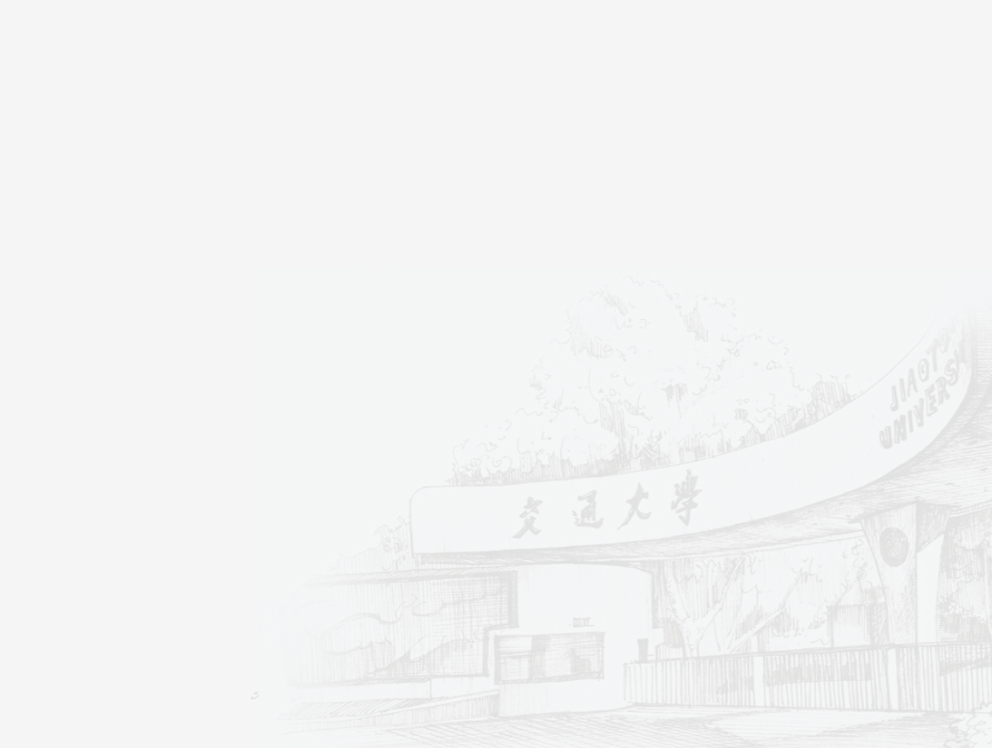
\includegraphics[height=\paperheight,width=\paperwidth]{background.png}}
\songti
\maketitle

\begin{frame}
    \frametitle{主要工作}
    \begin{itemize}
        \item 文献调研 \& 指定外文文献翻译; 
        \vspace{10pt}\item 相关背景知识学习; 
        \vspace{10pt}\item 聚类算法理论学习; 
        \vspace{10pt}\item 代码编写 \& 试验; 
        \vspace{10pt}\item 后续改进. 
    \end{itemize}
\end{frame}

\begin{frame}[shrink]
    \frametitle{文献调研}
    \vspace{10pt}
    通过约20篇的文献调研, 了解到NMO速度分析通常是通过以下几种方法: 
    
    \vspace{20pt}
    \begin{center}
        \begin{minipage}{.35\textwidth}
            \begin{itemize}
                \item 速度谱相似性; 

                \vspace{10pt}\item 局部地震斜率; 
                
                \vspace{10pt}\item 神经网络; 
                
                \vspace{10pt}\item 聚类. 
            \end{itemize}
        \end{minipage}
    \end{center}
\end{frame}

\begin{frame}[shrink]
    \frametitle{文献翻译}
    \vspace{20pt}
    对下列两篇文献进行了全文翻译. 

    \vspace{20pt}
    \fullcite{Zhang2016}\\约11000字
    
    \vspace{20pt}
    \fullcite{Rodriguez2014}\\约5000字
\end{frame}

\begin{frame}
    \frametitle{背景知识学习}
    由于地震勘探学背景知识的缺乏, 对此书籍的前四章进行了学习: 

    \vspace{15pt}
    \fullcite{Zhou2014}
\end{frame}

\begin{frame}
    \frametitle{聚类算法理论学习}

    对于EM算法, 变分推断, Dirichlet过程的相关文献进行了阅读, 并对于相关的公式和算法进行了推导. 

    \vspace{10pt}
    \fullcite{Blei2006}

    \vspace{10pt}
    \fullcite{Blei2017}
\end{frame}


\begin{frame}{代码编写}
    代码编写目前约950行, 实现了对地震数据进行读取、预处理、聚类、结果分析、曲线拟合、在原始道集上进行NMO校正的功能. 曲线拟合和NMO校正的代码目前还不完善. 

    \vspace{15pt}\url{https://github.com/Addasecond86/XJTU-Bachelor-Dissertation-Statistics-WangZehao/tree/main/codes}
\end{frame}

\begin{frame}
    \frametitle{试验结果}
    \begin{figure}[ht]
        \centering
        \subfigure[经过处理过后的最终聚类结果]{
            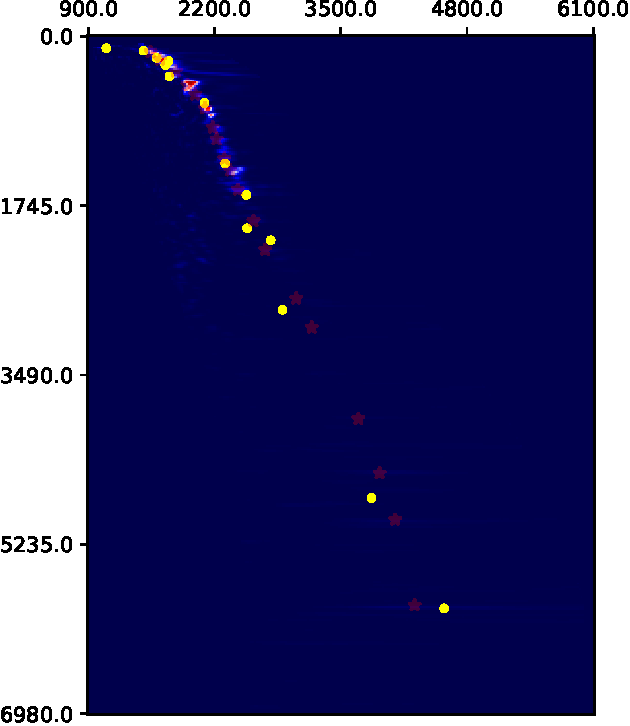
\includegraphics[height=6cm]{15_GMM_Dirichlet_TruePair_Centers_Real_n=35_n=9_CovType=diag_PriorType=dirichlet_process_Prior=0.03.pdf}
        }\ 
        \subfigure[曲线拟合结果]{
            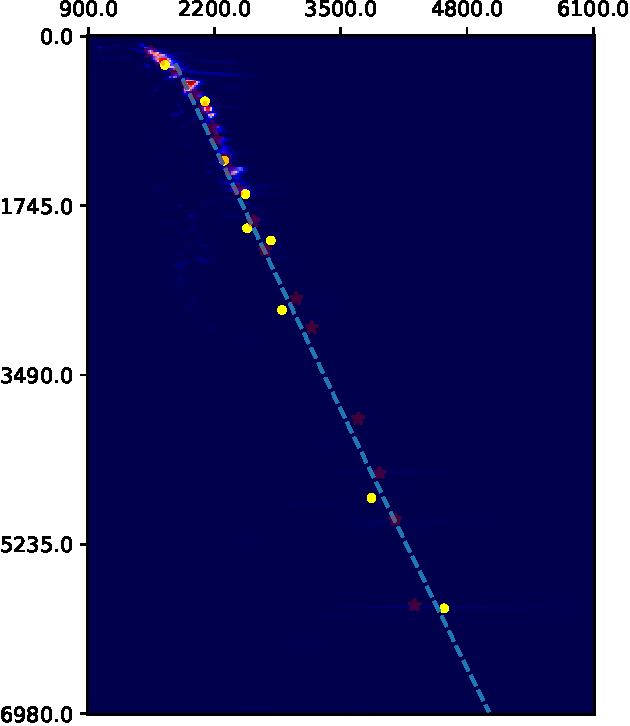
\includegraphics[height=6cm]{16_GMM_Dirichlet_FittingMethod=Square_Curve_TruePair_Centers_Real_n=35_n=10_CovType=diag_PriorType=dirichlet_process_Prior=0.03_NoCombine.pdf}
        }
    \end{figure}
\end{frame}

\begin{frame}
    \frametitle{试验结果}
    \begin{figure}[ht]
        \centering
        \subfigure[原始道集]{
            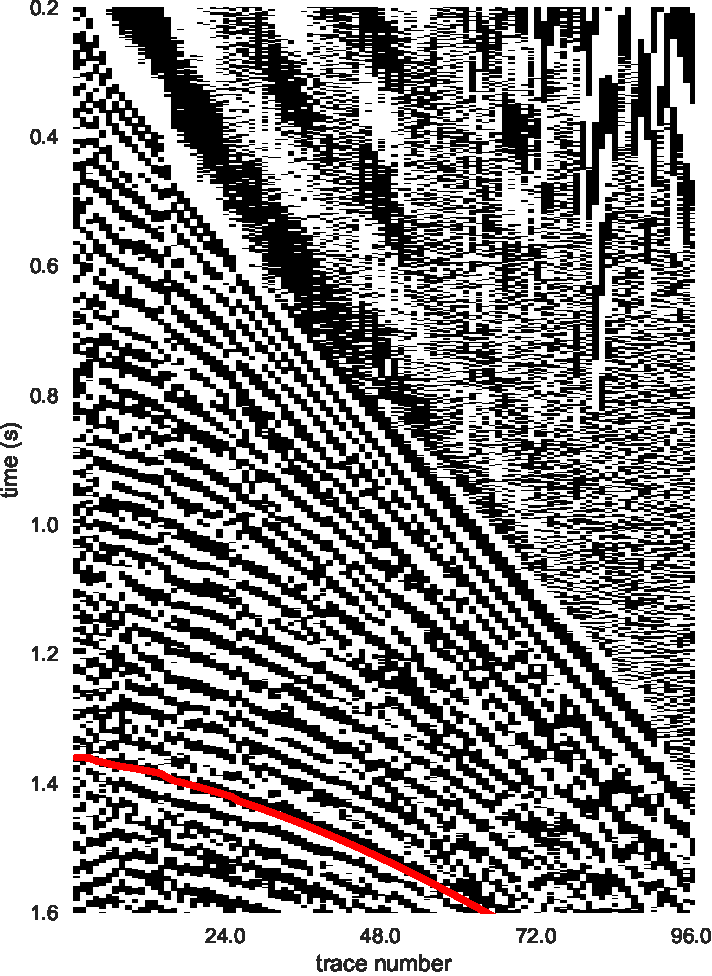
\includegraphics[height=6cm]{17_Show.pdf}
        }\ 
        \subfigure[动校正后结果]{
            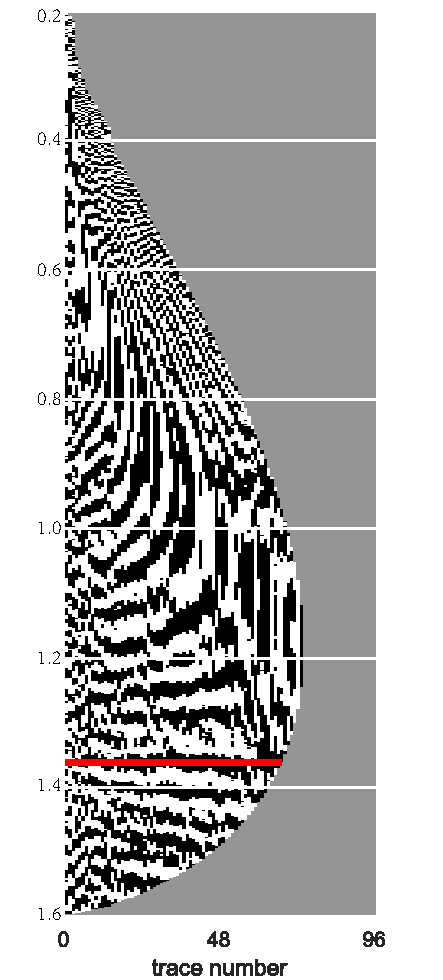
\includegraphics[height=6cm]{17_NMO.pdf}
        }
    \end{figure}
\end{frame}

\begin{frame}[shrink]
    \frametitle{后续改进}

    \vspace{20pt}
    后续改进主要考虑在以下几个方面: 
    
    \vspace{20pt}
    \begin{center}
        \begin{minipage}{.6\textwidth}
            \begin{enumerate}
                \vspace{10pt}\item 完善曲线拟合与NMO校正的代码
                \vspace{10pt}\item 探究更加有效剔除噪声的方法
                \vspace{10pt}\item 探究更为合理的曲线拟合方法
            \end{enumerate}
        \end{minipage}
    \end{center}
\end{frame}

\printbibliography

\begin{frame}[plain,standout]
    \LARGE \emph{谢谢观看}
\end{frame}

\end{document}
